\documentclass[12pt]{exam}

\usepackage{setspace}
\usepackage{listings}
\usepackage{subcaption}
\usepackage{float}
\usepackage{hyperref}
\usepackage{graphicx,wrapfig}
\usepackage{multirow}
\usepackage{amsmath}
\usepackage{bidihl}
\usepackage{tikz-uml}
%\usepackage{multicol}

\usepackage[margin=20mm]{geometry}
\usepackage{xepersian}
\settextfont{B Nazanin}

\newcommand{\class}{الگوها در مهندسی نرم افزار}

\hypersetup{
    colorlinks=true,
    linkcolor=blue,
    filecolor=magenta,      
    urlcolor=cyan,
    pdftitle={Overleaf Example},
    pdfpagemode=FullScreen,
    }
    
\singlespacing
\parindent 0ex

\lstset{
keywordstyle=\textbf,
identifierstyle=, 
stringstyle=\ttfamily,
commentstyle=\color{LimeGreen}, 
stringstyle=\ttfamily,
numberstyle=\footnotesize,
showstringspaces=false} 
\begin{document}


% -------------------------------------------------------
%  Thesis Information
% -------------------------------------------------------

\newcommand{\ThesisTitle}
{الگوها در سیستم های نهفته بی درنگ}
\newcommand{\ThesisAuthor}
{علی محسنی نژاد}
\newcommand{\ThesisSupervisor}
{دکتر رامان رامسین}
\newcommand{\ThesisDate}
{مرداد ۱۴۰۳}
\newcommand{\ThesisDepartment}
{دانشکده مهندسی کامپیوتر}
\newcommand{\ThesisUniversity}
{دانشگاه صنعتی شریف}

% -------------------------------------------------------
%  English Information
% -------------------------------------------------------

%\newcommand{\EnglishThesisTitle}{A Standard Template for Course Exercise}


\pagestyle{empty}

\begin{center}


\includegraphics[scale=0.2]{images/logo.png}

\vspace{0.5cm}
\ThesisUniversity \\[-0.3em]
\vspace{0.5cm}
\ThesisDepartment\\

\begin{large}
\vspace{0.5cm}


%\ThesisMajor

\end{large}

\vspace{1.5cm}

{عنوان:}\\[1.2em]
{\LARGE\textbf{\ThesisTitle}}\\ 
\vspace{1cm}
%\begin{latin}
%{\Large\textbf\EnglishThesisTitle}
%\end{latin}

\vspace{2cm}

{نویسنده}\\[.5em]
{\large\textbf{\ThesisAuthor}}

\vspace{1.5cm}

{استاد}\\[.5em]
{\large\textbf{\ThesisSupervisor}}

\vspace{1cm}



\vspace{2cm}

\ThesisDate

\end{center}

\newpage

\tableofcontents
% These commands set up the running header on the top of the exam pages
\pagestyle{head}
\firstpageheader{}{}{}
\runningheader{صفحه \thepage\ از \numpages}{}{\class}
\runningheadrule


\setlength\parindent{24pt}
\section{مقدمه}

\begin{RTL}
این گزارش به طور مفصل به توضیح الگوهای معرفی‌شده در مقالات و کتب مختلف
در حوزه سیستم‌های نهفته و بی‌درنگ می‌پردازد.
برای درک عمیق‌تر این الگوها، باید ابتدا مشخص شود که منظور
از سیستم‌های نهفته بی‌درنگ چیست.
سیستم‌های نهفته در بخش‌های زیادی از زندگی روزمره وجود دارند؛
به طور مثال سیستم‌های رادیویی، سیستم‌های ناوبری، سیستم‌های تصویربرداری.
به طور کلی یک سیستم نهفته را می‌توان اینگونه تعریف کرد،:
«یک سیستم کامپیوتری که به طور مشخص برای انجام یک کار در دنیای واقعی
تخصیص داده‌شده و هدف آن ایجاد یک محیط کامپیوتری
با کاربری عام نیست» \cite{ref1}.
یک دسته مهم از سیستم‌های نهفته، سیستم‌های بی‌درنگ هستند.
«سیستم‌های بی‌درنگ، سیستم‌هایی
هستند که در آن‌ها قیدهای زمانی مشخص باید برآورده شوند
تا سیستم بتواند به درستی کار کند» \cite{ref1}.
\end{RTL}

\begin{RTL}
حال که مفهوم سیستم‌های نهفته بی‌درنگ را دریافتیم، باید تعریفی از الگو در این سیستم‌ها
ارائه دهیم. منابع متنوع تعاریف متفاوتی از الگوها ارائه کرده‌اند و بسیاری از آن‌ها
این تعریف را به الگوهای طراحی محدود می‌کنند \cite{ref1}.
هدف این گزارش تقسیم‌بندی الگوهای نرم‌افزاری به طور کلی نیست و صرفا می‌خواهیم
الگوهای مورد استفاده در سیستم‌های نهفته و بی‌درنگ را بررسی کنیم.
\lr{Zalewski} \cite{ref2} می‌گوید:
«یک الگو یک مدل یا یک قالب نرم‌افزاری است که به فرایند ایجاد نرم‌افزار کمک می‌کند.»
این تعریف در عین سادگی، جامع است؛ به طوری که الگوهای طراحی، معماری و فرایندی
را در خود شامل می‌شود. با این حال این مقاله نیز مانند بسیاری از دیگر مقالات،
تعریف جدیدی از الگوها در سیستم‌های نهفته بی‌درنگ ارائه نکرده‌اند و برای تعریف آن به
تعریف \lr{Gamma} و دیگران \cite{ref3} از الگوهای طراحی ارجاع داده‌اند.
\end{RTL}

\begin{RTL}
\bidihl{
    ساختار گزارش و مطالبی که گفته می‌شود.
}
\end{RTL}


\section{\lr{Survey}}
\subsection{الگوهای طراحی برای دسترسی به سخت‌افزار}
\begin{RTL}
نرم‌افزارهای نهفته بر روی یک بستر سخت‌افزاری مستقر می‌شوند و معمولا بسیاری از قابلیت‌های
آن‌ها ملزم به ارتباط با سخت‌افزار می‌شود. به همین دلیل \lr{Douglass}
\cite{ref1} یک دسته از الگوها را با عنوان الگوهای دسترسی به سخت‌افزار
معرفی می‌کند.
\end{RTL}
\subsubsection{الگوی \lr{Hardware Proxy}}
\label{HWProxySec}
\begin{RTL}
این الگو \cite{ref1} با ایجاد یک رابط روی یک جزء سخت‌افزاری، یک دسترسی
مستقل از پیچیدگی‌های اتصال به سخت‌افزار برای کلاینت ایجاد می‌کند.
این الگو با معرفی یک کلاس به نام پروکسی بین سخت‌افزار و کلاینت،
باعث می‌شود که تمامی عملیات وابسته به سخت‌افزار در پروکسی انجام شود
و در صورت تغییر در سخت‌افزار، هیچ تغییری به کلاینت تحمیل نشود.
در این الگو بر روی یک جزء سخت‌افزاری، یک پروکسی قرار گرفته و
کلاینت‌های متعدد می‌توانند از آن سرویس بگیرند. لازم به ذکر است که ارتباط پروکسی
و سخت‌افزار بر پایه یک «رابط قابل آدرس‌دهی توسط نرم‌افزار» است. 
دیاگرام کلاس این الگو در شکل \ref{HWProxyClassDiag} رسم شده‌است.
\end{RTL}
\begin{figure}[h!]
\centering
\begin{tikzpicture}
\lr{
  \umlclass{HardwareProxy}{
    device\_address
  }{
    initialize()\\
    configure()\\
    disable()\\
    access()\\
    mutate()
  }
  \umlclass[y=-6]{HardwareDevice}{
    \lr{}
  }{}
  \umlclass[x=5]{ProxyClient}{
    \lr{}
  }{}
\umlassoc[mult1=1, mult2=1]{HardwareProxy}{HardwareDevice}
\umluniassoc[mult1=1..*, mult2=1]{ProxyClient}{HardwareProxy}
}
\end{tikzpicture}
\caption{دیاگرام کلاس \lr{Hardware Proxy}}
\label{HWProxyClassDiag}
\end{figure}
\begin{RTL}
همانطور که در شکل \ref{HWProxyClassDiag} دیده می‌شود، کلاس پروکسی توابع
مشخصی را در اختیار کلاینت‌ها قرار می‌دهد\footnote{توابع دیگری نیز در \cite{ref1}
گفته‌شده ولی اینجا تنها توابع \lr{public} کلاس پروکسی را بررسی می‌کنیم.}.
توضیحات مربوط به هر یک از توابع کلاس پروکسی در شکل زیر داده شده‌است:
\begin{itemize}
  \item \lr{initialize}:
  این تابع برای آماده‌سازی اولیه ارتباط با سخت‌افزار استفاده می‌شود و معمولا تنها یک بار
  صدا زده می‌شود.
  \item \lr{configure}:
  این تابع برای ارسال تنظیمات برای سخت‌افزار استفاده می‌شود. معمولا باید در سخت‌افزار
  تنظیماتی قرار داده‌شود که آن را قابل استفاده کند.
  \item \lr{disable}:
  این تابع برای غیرفعال‌کردن سخت‌افزار به صورت امن استفاده می‌شود.
  \item \lr{access}:
  این تابع برای دریافت اطلاعات از طرف سخت‌افزار استفاده می‌شود.
  \item \lr{mutate}:
  این تابع برای فرستادن اطلاعات به سمت سخت‌افزار استفاده می‌شود.
\end{itemize}
\end{RTL}
\begin{RTL}
این الگو بسیار رایج است و مزایای کپسوله‌سازی رابط سخت‌افزار و جزئیات
کدگذاری را فراهم می‌کند، به طوری که تغییرات رابط سخت‌افزار بدون نیاز به
تغییر در کلاینت‌ها انجام می‌شود. این کپسوله‌سازی می‌تواند تأثیر منفی
بر عملکرد زمان اجرا داشته باشد، زیرا کاربران از فرمت اصلی داده‌ها آگاه
نیستند. با این حال، آگاهی کلاینت‌ها از جزئیات کدگذاری باعث پیچیدگی
در نگه‌داشت سیستم می‌شود.
\end{RTL}
\subsubsection{الگوی \lr{Hardware Adapter}}
\label{HWAdapterSec}
\begin{RTL}
این الگو \cite{ref1} مشابه الگوی \lr{Adapter} که \lr{Gamma} و دیگران
\cite{ref3} معرفی کرده‌اند تعریف شده. استفاده از این الگو این اجازه را
می‌دهد که کلاینتی که انتظار یک رابط خاص با سخت‌افزار را دارد، بتواند با
سخت‌افزارهای مختلف بدون این‌که متوجه تفاوت‌های آن‌ها شود ارتباط بگیرد.
این الگو روی ساختار \nameref{HWProxySec} بنا شده‌است و
دیاگرام کلاس آن در شکل \ref{HWAdapterClassDiag} ترسیم شده‌است.
\end{RTL}
\begin{figure}[h!]
\centering
\begin{tikzpicture}
\lr{
    \umlclass{HardwareProxy}{
    device\_address
    }{
    initialize()\\
    configure()\\
    disable()\\
    access()\\
    mutate()
    }
    \umlclass[y=-6]{HardwareDevice}{
    \lr{}
    }{}
    \umlclass[x=6]{HardwareAdapter}{
    \lr{}
    }{
        clientService1() \\
        clientService2()
    }
    \umlinterface[x=6, y=4]{HardwareInterfaceToClient}{}{
        \umlvirt{clientService1()} \\
        \umlvirt{clientService2()}
    }
    \umlclass[x=13, y=4]{AdapterClient}{
        \lr{}
    }{}
\umlassoc[mult1=1, mult2=1]{HardwareProxy}{HardwareDevice}
\umluniassoc[mult1=1..*, mult2=1]{HardwareAdapter}{HardwareProxy}
\umlimpl[]{HardwareAdapter}{HardwareInterfaceToClient}
\umlassoc[mult1=1, mult2=1]{AdapterClient}{HardwareInterfaceToClient}
}
\end{tikzpicture}
\caption{دیاگرام کلاس \lr{Hardware Adapter}}
\label{HWAdapterClassDiag}
\end{figure}
\begin{RTL}
همانطور که در شکل \ref{HWAdapterClassDiag} دیده می‌شود،
کلاس کلاینت سرویس‌های مورد انتظار خود را از رابط
\lr{HardwareInterfaceToClient} انتظار دارد.
در این ساختار، کلاس آداپتور، سرویس‌های مورد انتظار کلاینت را به سرویس‌های ارائه‌شده
از طرف سخت‌افزار ترجمه می‌کند. این کار اجازه می‌دهد که در صورت تغییر سخت‌افزار
(و متناظرا پروکسی)، تنها با ایجاد پیاده‌سازی جدید برای رابط آداپتور، نیازی به تغییر
در کلاینت نباشد.
\end{RTL}
\begin{RTL}
استفاده از این الگو اجازه می‌دهد پروکسی‌های سخت‌افزار و دستگاه‌های مرتبط در
برنامه‌های مختلف بدون تغییر استفاده شوند و برنامه‌های موجود نیز بدون
تغییر از دستگاه‌های سخت‌افزاری مختلف استفاده کنند.
\lr{Adapter} به‌عنوان پل ارتباطی بین پروکسی سخت‌افزار
و برنامه عمل می‌کند، که تغییر یا استفاده مجدد از دستگاه‌های سخت‌افزاری را آسان‌تر،
سریع‌تر و کم‌خطاتر می‌سازد. هزینه استفاده از این الگو افزایش سطح انتزاع
و کاهش اندک عملکرد زمان اجرا است.
\end{RTL}
\subsubsection{الگوی \lr{Mediator}}
\label{HWMediatorSec}
\begin{RTL}
این الگو با معرفی یک کلاس میانجی‌گر بین چند کلاس همکار، کمک می‌کند که چند
سخت‌افزار را با هم مدیریت کند. ساختار این الگو در شکل \ref{HWMediatorClassDiag}
ترسیم شده‌است.
\end{RTL}
\begin{figure}[h!]
\centering
\begin{tikzpicture}
\lr{
    \umlclass{Mediator}{}{}
    \umlinterface[x=5]{CollaboratorInterface}{}{}
    \umlclass[x=5, y=-3]{SpecificCollaborator}{}{}
\umluniassoc[mult2=1]{CollaboratorInterface}{Mediator}
\umlimpl{SpecificCollaborator}{CollaboratorInterface}
\umluniassoc[geometry=|-, mult2=1..*, pos2=1.8]{Mediator}{SpecificCollaborator}
}
\end{tikzpicture}
\caption{دیاگرام کلاس \lr{Mediator}}
\label{HWMediatorClassDiag}
\end{figure}
\begin{RTL}
همانطور که در شکل مشخص است، کلاس میانجی با هر یک از کلاس‌های همکار ارتباط دارد.
این ارتباط به این شکل است که کلاس میانجی تمامی پیاده‌سازی‌های رابط همکار را می‌شناسد
و با آن‌ها ارتباط دارد. این کلاس‌ها خودشان نیز همانطور که نشان‌داده شده،
میانجی را می‌شناسند و با آن ارتباط دارند.
هر یک از کلاس‌های همکار، با سخت‌افزار در ارتباط هستند و حتی می‌توانند خود یک پروکسی
باشند (\nameref{HWProxySec}).
ولی به هر صورت در این الگو برای ارتباط با یکدیگر، باید برای میانجی سیگنال
بفرستند و میانجی وظیفه ارتباطات بین همکارها را دارد (با ایجاد ارتباط غیر مستقیم).
به طور کلی فرایندهایی که در آن
استفاده از چند سخت‌افزار و نیاز است، توسط میانجی کنترل می‌شود.
\end{RTL}
\subsubsection{الگوی \lr{Observer}}
\label{HWObserverSec}
\begin{RTL}
یکی از پرکاربردترین الگوها در حوزه سیستم‌های نهفته، الگوی \lr{Observer} \cite{ref1} است.
این الگو به شیء‌های برنامه این اجازه را می‌دهد که به یک شی‌ء دیگر برای دریافت
اطلاعات گوش دهند. این به این معنی است که اگر یک کلاینت به دنبال دریافت
داده از یک سرور است، به جای این که هر دفعه درخواست دریافت داده‌ها را برای
سرور بفرستد، برای آن سرور درخواست عضویت فرستاده و سرور هرگاه که داده‌های جدید
در دسترس بودند، آن‌ها را برای کلاینت‌های عضوشده بفرستد. یکی از مهم‌ترین کاربردهای
این الگو در دریافت داده‌ها از سنسورها است.
یکی از قابلیت‌های خوب این الگو این است که کلاینت‌ها می‌توانند در زمان اجرای برنامه
عضویت خود را قطع یا ایجاد کنند. در شکل \ref{HWObserverClassDiag}
دیاگرام کلاس این الگو را می‌بینیم.
\end{RTL}
\begin{figure}[h!]
\centering
\begin{tikzpicture}
\lr{
    \umlinterface{AbstractClient}{}{
        \lr{accept(d: Datum)}
    }
    \umlclass[y=-3]{ConcreteClient}{}{}
    \umlclass[x=4, y=3]{Datum}{}{}
    \umlinterface[x=8]{AbstractSubject}{}{
        \lr{subscribe(a: acceptPtr)} \\
        \lr{unsubscribe(a: acceptPtr)} \\
        \lr{notify()}
    }
    \umlclass[x=8, y=-3]{ConcreteSubject}{}{}
    \umlclass[x=13, y=-3]{NotificationHandle}{
        \lr{aPtr: acceptPtr}
    }{}
\umluniassoc[geometry=|-, attr2=1|itsDatum, pos2=1.9, align2=left]{AbstractSubject}{Datum}
\umluniassoc[geometry=|-, attr2=1|itsDatum, pos2=1.9, align2=right]{AbstractClient}{Datum}
\umluniassoc[attr2=1|itsAbstractSubject, pos2=1, align2=right]{AbstractClient}{AbstractSubject}
\umlimpl{ConcreteSubject}{AbstractSubject}
\umlimpl{ConcreteClient}{AbstractClient}
\umlunicompo[geometry=-|, attr2=MAX\_SUBS|, pos2=1.9]{AbstractSubject}{NotificationHandle}
}
\end{tikzpicture}
\caption{دیاگرام کلاس \lr{Observer}}
\label{HWObserverClassDiag}
\end{figure}
\begin{RTL}
در این ساختار کلاینت‌ها با فرستادن یک اشاره‌گر به کلاس سابجکت، درخواست عضویت برای 
سرویس می‌فرستند. کلاس سابجکت نیز با ذخیره‌کردن اشاره‌گرهای مختلف از طرف کلاینت‌ها
زمانی که داده جدید آماده می‌شود، با فراخوانی تابع \lr{notify}، تابع \lr{accept}
که اشاره‌گرهایش را در \lr{NotificationHandle} قرار داده، با پاس دادن
ورودی به فرمت \lr{Datum} صدا می‌زند. اینگونه این داده برای تمامی کلاینت‌های
عضو سرویس فرستاده می‌شود.
کلاینت‌ها می‌توانند در حین اجرای برنامه، عضویت خود برای سرویس را لغو کنند.
دقت شود که خود کلاس‌‌های سابجکت
معمولا از نوع پروکسی هستند (\nameref{HWProxySec}).
\end{RTL}
\begin{RTL}
این الگو فرآیند توزیع داده‌ها به مجموعه‌ای از کلاینت‌ها را که ممکن است
در زمان طراحی مشخص نباشند، ساده می‌کند و مدیریت داینامیک
لیست کلاینت‌های علاقه‌مند در زمان اجرا را فراهم می‌کند.
این الگو رابطه اصلی کلاینت-سرور را حفظ می‌کند و از طریق مکانیزم
اشتراک‌گذاری، انعطاف‌پذیری در زمان اجرا ارائه می‌دهد.
بهره‌وری محاسباتی حفظ می‌شود زیرا کلاینت‌ها تنها زمانی که
مناسب است به‌روزرسانی می‌شوند؛ سیاست رایج این است
که مشتریان در زمان تغییر داده‌ها به‌روزرسانی شوند، اما هر
سیاست مناسب دیگری نیز می‌تواند اعمال شود.
\end{RTL}
\subsubsection{الگوی \lr{Debouncing}}
\label{HWDebouncingSec}
\begin{RTL}
در سخت‌افزار بسیاری از ورودی‌ها به صورت دکمه‌ها و سوییچ‌هایی هستند که بر اثر ایجاد
اتصال دو فلز با یکدیگر، باعث فعال‌شدن یک پایه شده و آغازگر یک عملیات در نرم‌افزار
نهفته هستند. اتصال این دو فلز با یکدیگر دارای تعدادی حالت میانی است. به این صورت
که اتصال با کمی لرزش همراه بوده و اتصال برای چند میلی‌ثانیه چند بار قطع و وصل
می‌شود. این قطع و وصل شدن، باعث می‌شود که نتوانیم حالت فعلی سخت‌افزار را به درستی
در نرم‌افزار ضبط کنیم.
\end{RTL}
\begin{RTL}
این الگو \cite{ref1} به ما کمک می‌کند که با صبرکردن برای یک مدت کوتاه، مقدار ورودی را
زمانی که پایدار شده‌است بخوانیم. با این کار دغدغه معتبر بودن مقدار خوانده‌شده را
در کلاینت نخواهیم داشت. دیاگرام کلاسی این الگو در شکل \ref{HWDebouncingClassDiag}
نمایش داده شده‌است.
\end{RTL}
\begin{figure}[h!]
\centering
\begin{tikzpicture}
\lr{
    \umlclass{BouncingDevice}{
        \lr{deviceState}
    }{
        \lr{sendEvent()} \\
        \lr{getState()}
    }
    \umlclass[x=7]{Debouncer}{
        \lr{oldState}
    }{
        \lr{eventReceive()}
    }
    \umlclass[x=7, y=-4]{ApplicationClient}{}{
        \lr{deviceEventReceive(dState)}
    }
    \umlclass[x=7, y=4]{DebouncingTimer}{}{
        \lr{delay(delayTime)}
    }
\umlassoc[mult1=1, mult2=1]{Debouncer}{BouncingDevice}
\umluniassoc[attr2=1|itsApplicationClient]{Debouncer}{ApplicationClient}
\umluniassoc[attr2=itsDebouncingTimer|1]{Debouncer}{DebouncingTimer}
}
\end{tikzpicture}
\caption{دیاگرام کلاس \lr{Debouncing}}
\label{HWDebouncingClassDiag}
\end{figure}
\begin{RTL}
در این ساختار، \lr{BouncingDevice} همان سخت‌افزار مورد بررسی است.
تابع \lr{sendEvent} می‌تواند یک نوع اینتراپت سخت‌افزاری باشد که نرم‌افزار را
از تغییر در سخت‌افزار باخبر می‌سازد و \lr{getState} می‌تواند یک عملیات
خواندن از حافظه باشد.
کلاس \lr{Debouncer} وظیفه ارائه حالت پایدار سخت‌افزار به کلاینت را دارد.
این کار با استفاده از یک کلاس زمان‌سنج انجام می‌شود که با ایجاد یک تاخیر نرم‌افزاری
تا پایدارشدن شرایط خروجی سخت‌افزار، خواندن حالت سخت‌افزار را به تعویق می‌اندازد.
\end{RTL}
\subsubsection{الگوی \lr{Interrupt}}
\label{HWInterruptSec}
\begin{RTL}
یکی از واحدهای مهم در سیستم‌های سخت‌افزاری، واحد \lr{Interrupt} است.
\lr{Interrupt} برای هندل‌کردن وقایعی است که توسط سخت‌افزار جرقه زده می‌شوند.
زمانی که یک \lr{interrupt} رخ می‌دهد، نرم‌افزار فرایند کاری اصلی خود را متوقف
کرده و یک فرایند رسیدگی به \lr{interrupt} اتفاق‌افتاده آغاز می‌شود. با انجام
این فرایند و رسیدگی به \lr{interrupt}، فرایند اصلی نرم‌افزار دوباره از سر گرفته
می‌شود. ساختار این الگو در شکل \ref{HWInterruptClassDiag}
نمایش داده شده‌است.
\end{RTL}
\begin{figure}[h!]
\centering
\begin{tikzpicture}
\lr{
    \umlclass{InterruptVectorTable <<File>>}{
        \lr{ISRAddress: vectorPtr[]}
    }{}
    \umlclass[x=7]{InterruptHandler}{
        \lr{oldVectors: vectorPtr}
    }{
        \lr{install()}\\
        \lr{deinstall()}\\
        \lr{handleInterrupt1()}\\
        \lr{handleInterrupt2()}\\
        \lr{handleInterrupt3()}\\
        \lr{handleInterrupt4()}
    }
    \umlclass[x=3, y=-5]{vectorPtr <<Type>>}{
        \lr{void (*vectorPtr)(void)}
    }{}
\umluniassoc[mult2=1]{InterruptHandler}{InterruptVectorTable <<File>>}
\umldep{InterruptHandler}{vectorPtr <<Type>>}
\umldep{InterruptVectorTable <<File>>}{vectorPtr <<Type>>}
}
\end{tikzpicture}
\caption{دیاگرام کلاس \lr{Interrupt}}
\label{HWInterruptClassDiag}
\end{figure}
\begin{RTL}
در این الگو، کلاس \lr{InterruptHandler} کار اصلی را انجام می‌دهد.
این کلاس دارای بردار \lr{Interrupt}هاست.
با فراخوانی تابع \lr{install} می‌توان این بردار را با یک بردار جدید جایگزین‌کرد.
این بردار در اصل تعدادی اشاره‌گر به توابعی است که در صورت بروز \lr{Interrupt}
باید فراخوانی شوند. با تابع \lr{deinstall} نیز می‌توان بردار را به حالت قبلی
برگرداند. فایل \lr{InterruptVectorTable} شامل یک لیست از
اشاره‌گرها به توابع \lr{Interrupt Service Routine} است.
و \lr{vectorPtr} صرفا یک نوع اشاره‌گر به تابع است که از نوع آن در
\lr{InterruptVectorTable} استفاده شده‌است.
\end{RTL}
\subsubsection{الگوی \lr{Polling}}
\label{HWPollingSec}
\begin{RTL}
این الگو \cite{ref1} یک روش دیگر برای دریافت داده‌ها
از سنسورها است و زمانی استفاده می‌شود که
استفاده از \nameref{HWInterruptSec} ممکن نیست یا این که
داده‌هایی که می‌خواهیم ضبط کنیم آن قدر اضطراری نیستند و می‌توان برای دریافت آن‌ها
صبر کرد. عملکرد این الگو به این صورت است که با سرکشی‌کردن به صورت دوره‌ای داده‌ها
را دریافت می‌کنیم. حال این الگو در دو شکل بیان می‌شود: سرکشی داده‌ها به صورت
دوره‌ای و به صورت فرصتی.
در نوع اول با استفاده از یک تایمر، در زمان‌های مشخصی، برای دریافت داده‌های جدید
سرکشی می‌کنیم که ساختار کلاسی آن نیز
در شکل \ref{HWPeriodicPollingClassDiag} نشان داده شده‌است.
در نوع دوم زمانی عمل سرکشی را انجام می‌دهیم که برای سیستم ممکن باشد و
قیدهای زمانی سیستم به ما این اجاره را بدهد. ساختار کلاسی این نوع نیز در شکل
\ref{HWOpportunisticPollingClassDiag} رسم شده‌است.
\end{RTL}
\begin{figure}[h!]
\centering
\begin{tikzpicture}
\lr{
    \umlclass{Device}{
        \lr{data}\\
        \lr{deviceState}
    }{
        \lr{getData()} \\
        \lr{getState()}
    }
    \umlclass[x=8]{PeriodicPoller}{
        \lr{pollTime}
    }{
        \lr{startPolling()}\\
        \lr{stopPolling()}\\
        \lr{poll()}\\
        \lr{setPollTime()}
    }
    \umlclass[x=8, y=-5]{PollDataClient}{}{
        \lr{handleData()}\\
        \lr{handleDeviceState()}
    }
    \umlclass[x=8, y=6]{PollTimer}{
        \lr{oldVector}
    }{
        \lr{installInterruptHandler()}\\
        \lr{removeInterruptHandler()}\\
        \lr{startTimer()}\\
        \lr{stopTimer()}\\
        \lr{handleTimerInterrupt()}
    }
\umluniassoc[mult2=MAX\_POLL\_DEVICES, pos2=0.5]{PeriodicPoller}{Device}
\umluniassoc[mult2=MAX\_POLL\_DEVICES]{PeriodicPoller}{PollDataClient}
\umlassoc[mult1=1, mult2=1]{PeriodicPoller}{PollTimer}
}
\end{tikzpicture}
\caption{دیاگرام کلاس \lr{Periodic Polling}}
\label{HWPeriodicPollingClassDiag}
\end{figure}

\begin{figure}[h!]
\centering
\begin{tikzpicture}
\lr{
    \umlclass{Device}{
        \lr{data}\\
        \lr{deviceState}
    }{
        \lr{getData()} \\
        \lr{getState()}
    }
    \umlclass[x=8]{OpportunisticPoller}{}{
        \lr{poll()}
    }
    \umlclass[x=8, y=-5]{PollDataClient}{}{
        \lr{handleData()}\\
        \lr{handleDeviceState()}
    }
    \umlclass[x=8, y=6]{ApplicationProcessingElement}{}{
        \lr{applicationFunction()}
    }
\umluniassoc[mult2=MAX\_POLL\_DEVICES, pos2=0.5]{OpportunisticPoller}{Device}
\umluniassoc[mult2=MAX\_POLL\_DEVICES]{OpportunisticPoller}{PollDataClient}
\umluniassoc[mult2=1]{ApplicationProcessingElement}{OpportunisticPoller}
}
\end{tikzpicture}
\caption{دیاگرام کلاس \lr{Opportunistic Polling}}
\label{HWOpportunisticPollingClassDiag}
\end{figure}
\begin{RTL}
در این الگو کلاس \lr{Device} همان سخت‌افزار/حافظه/... هست که
می‌خواهیم داده‌هایش را دریافت کنیم. کلاس \lr{PollDataClient} نیز
کلاینتی است که می‌خواهد داده‌های \lr{Device} را دریافت کند.
در ساختار شکل \ref{HWPeriodicPollingClassDiag}، کلاس
\lr{PeriodicPoller} با سرکشی از \lr{Device} داده‌های
آن را دریافت می‌کند. این سرکشی زمانی انجام می‌شود که کلاس \lr{PollTimer}
تابع \lr{poll} را از \lr{PeriodicPoller} صدا بزند.
زمانی که فرمان \lr{startPolling} به بیاید، تایمر کار خود را شروع
می‌کند و در هر \lr{Interrupt}ی که تایمر می‌خورد، تابع \lr{poll} را
صدا می‌زند. با فراخوانی تابع \lr{stopPolling}، تایمر متوقف می‌شود.
در ساختار \ref{HWOpportunisticPollingClassDiag} تفاوت
در این است که تابع \lr{poll} زمانی صدا زده می‌شود که کلاس
\lr{ApplicationProcessingElement} بخواهد. یعنی زمانی که این
کلاس در فرایندهای خود لازم می‌بیند که لازم است داده‌های جدید از \lr{Device}
گرفته‌شود، این تابع صدا زده می‌شود.
\end{RTL}
\begin{RTL}
\lr{polling} ساده‌تر از راه‌اندازی و استفاده از
\lr{ISR} (\nameref{HWInterruptSec}) است، هرچند \lr{Polling}
دوره‌ای معمولاً با \lr{ISR} مرتبط با تایمر \lr{Polling} انجام می‌شود.
\lr{Polling} می‌تواند وضعیت بسیاری از دستگاه‌ها را همزمان بررسی کند
اما معمولاً نسبت به وقفه‌ها کمتر به موقع است. اگر داده‌ها سریع‌تر از
زمان \lr{Polling} برسند، داده‌ها از دست خواهند رفت.
این موضوع در بسیاری از برنامه‌ها مشکلی ایجاد نمی‌کند اما در برخی دیگر
می‌تواند فاجعه‌بار باشد.
\end{RTL}
\section{الگوهای طراحی برای دسترسی به سخت‌افزار}
\begin{RTL}
نرم‌افزارهای نهفته بر روی یک بستر سخت‌افزاری مستقر می‌شوند و معمولا بسیاری از قابلیت‌های
آن‌ها ملزم به ارتباط با سخت‌افزار می‌شود. به همین دلیل \lr{Douglass}
\cite{ref1} یک دسته از الگوها را با عنوان الگوهای دسترسی به سخت‌افزار
معرفی می‌کند.
\end{RTL}
\subsection{الگوی \lr{Hardware Proxy}}
\label{HWProxySec}
\begin{RTL}
این الگو با ایجاد یک رابط روی یک جزء سخت‌افزاری، یک دسترسی
مستقل از پیچیدگی‌های اتصال به سخت‌افزار برای کلاینت ایجاد می‌کند.
این الگو با معرفی یک کلاس به نام پروکسی بین سخت‌افزار و کلاینت،
باعث می‌شود که تمامی عملیات وابسته به سخت‌افزار در پروکسی انجام شود
و در صورت تغییر در سخت‌افزار، هیچ تغییری به کلاینت تحمیل نشود.
در این الگو بر روی یک جزء سخت‌افزاری، یک پروکسی قرار گرفته و
کلاینتان متعدد می‌توانند از آن سرویس بگیرند. لازم به ذکر است که ارتباط پروکسی
و سخت‌افزار بر پایه یک «رابط قابل آدرس‌دهی توسط نرم‌افزار» است. 
دیاگرام کلاس این الگو در شکل \ref{HWProxyClassDiag} رسم شده‌است.
\end{RTL}
\begin{figure}[h!]
\centering
\begin{tikzpicture}
\lr{
  \umlclass{HardwareProxy}{
    device\_address
  }{
    initialize()\\
    configure()\\
    disable()\\
    access()\\
    mutate()
  }
  \umlclass[y=-6]{HardwareDevice}{
    \lr{}
  }{}
  \umlclass[x=5]{ProxyClient}{
    \lr{}
  }{}
\umlassoc[mult1=1, mult2=1]{HardwareProxy}{HardwareDevice}
\umluniassoc[mult1=1..*, mult2=1]{ProxyClient}{HardwareProxy}
}
\end{tikzpicture}
\caption{دیاگرام کلاس \lr{Hardware Proxy}}
\label{HWProxyClassDiag}
\end{figure}
\begin{RTL}
همانطور که در شکل \ref{HWProxyClassDiag} دیده می‌شود، کلاس پروکسی توابع
مشخصی را در اختیار کلاینت‌ها قرار می‌دهد\footnote{توابع دیگری نیز در \cite{ref1}
گفته‌شده ولی اینجا تنها توابع \lr{public} کلاس پروکسی را بررسی می‌کنیم.}.
توضیحات مربوط به هر یک از توابع کلاس پروکسی در شکل زیر داده شده‌است:
\begin{itemize}
  \item \lr{initialize}:
  این تابع برای آماده‌سازی اولیه ارتباط با سخت‌افزار استفاده می‌شود و معمولا تنها یک بار
  صدا زده می‌شود.
  \item \lr{configure}:
  این تابع برای ارسال تنظیمات برای سخت‌افزار استفاده می‌شود. معمولا باید در سخت‌افزار
  تنظیماتی قرار داده‌شود که آن را قابل استفاده کند.
  \item \lr{disable}:
  این تابع برای غیرفعال‌کردن سخت‌افزار به صورت امن استفاده می‌شود.
  \item \lr{access}:
  این تابع برای دریافت اطلاعات از طرف سخت‌افزار استفاده می‌شود.
  \item \lr{mutate}:
  این تابع برای فرستادن اطلاعات به سمت سخت‌افزار استفاده می‌شود.
\end{itemize}
\end{RTL}
\subsection{الگوی \lr{Hardware Adapter}}
\label{HWAdapterSec}
\begin{RTL}
این الگو مشابه الگوی \lr{Adapter} که \lr{Gamma} و دیگران
\cite{ref3} معرفی کرده‌اند تعریف شده. استفاده از این الگو این اجازه را
می‌دهد که کلاینتی که انتظار یک رابط خاص با سخت‌افزار را دارد، بتواند با
سخت‌افزارهای مختلف بدون این‌که متوجه تفاوت‌های آن‌ها شود ارتباط بگیرد.
این الگو روی ساختار \nameref{HWProxySec} بنا شده‌است و
دیاگرام کلاس آن در شکل \ref{HWAdapterClassDiag} ترسیم شده‌است.
\end{RTL}
\begin{figure}[h!]
\centering
\begin{tikzpicture}
\lr{
    \umlclass{HardwareProxy}{
    device\_address
    }{
    initialize()\\
    configure()\\
    disable()\\
    access()\\
    mutate()
    }
    \umlclass[y=-6]{HardwareDevice}{
    \lr{}
    }{}
    \umlclass[x=6]{HardwareAdapter}{
    \lr{}
    }{
        clientService1() \\
        clientService2()
    }
    \umlinterface[x=6, y=4]{HardwareInterfaceToClient}{}{
        \umlvirt{clientService1()} \\
        \umlvirt{clientService2()}
    }
    \umlclass[x=13, y=4]{AdapterClient}{
        \lr{}
    }{}
\umlassoc[mult1=1, mult2=1]{HardwareProxy}{HardwareDevice}
\umluniassoc[mult1=1..*, mult2=1]{HardwareAdapter}{HardwareProxy}
\umlimpl[]{HardwareAdapter}{HardwareInterfaceToClient}
\umlassoc[mult1=1, mult2=1]{AdapterClient}{HardwareInterfaceToClient}
}
\end{tikzpicture}
\caption{دیاگرام کلاس \lr{Hardware Adapter}}
\label{HWAdapterClassDiag}
\end{figure}
\begin{RTL}
همانطور که در شکل \ref{HWAdapterClassDiag} دیده می‌شود،
کلاس کلاینت سرویس‌های مورد انتظار خود را از رابط
\lr{HardwareInterfaceToClient} انتظار دارد.
در این ساختار، کلاس آداپتور، سرویس‌های مورد انتظار کلاینت را به سرویس‌های ارائه‌شده
از طرف سخت‌افزار ترجمه می‌کند. این کار اجازه می‌دهد که در صورت تغییر سخت‌افزار
(و متناظرا پروکسی)، تنها با ایجاد پیاده‌سازی جدید برای رابط آداپتور، نیازی به تغییر
در کلاینت نباشد.
\end{RTL}



% \umlassoc[geometry=-|-,
%   arg1=tata,
%   mult1=*,
%   pos1=1.3,
%   arg2=toto,
%   align1=bottom,
%   mult2=1,
%   pos2=1.7,
%   align2=top
% ]{Proxy}{Hardware}
\subsection{الگوهای طراحی برای ماشین‌های حالت}
\begin{RTL}
این دسته از الگوها که توسط \lr{Douglass} در \cite{ref1}
معرفی شده‌است، الگوهایی هستند که براساس ماشین‌های حالت ساخته شده‌اند.
\end{RTL}
\subsubsection{الگوی \lr{Single Event Receptor}}
\label{smSingleEvRecSec}
\begin{RTL}
این الگو یک دریافت‌کننده رویداد را به کلاینت‌ها عرضه می‌کند که می‌تواند رویدادهای
سنکرون و آسنکرون را دریافت کند. در این الگو، ورودی این دریافت‌کنند علاوه بر
نوع رویدادی که رخ‌داده‌است، باید دارای داده‌های مربوط به رویداد نیز باشد. 
\end{RTL}
\subsubsection{الگوی \lr{Multiple Event Receptor}}
\subsubsection{الگوی \lr{State Table}}
\subsubsection{الگوی \lr{State}}
\label{smStateSec}
\begin{RTL}
این الگو \cite{ref1} با واسپاری حالت سیستم به یک شیء
مجزا، وظیفه مدیریت حالت را به آن می‌دهد. در این الگو، تمامی رویدادهای دریافتی
به این شیء پاس داده می‌شوند و او با توجه به این که حالت بعدی را می‌شناسد،
خود را با شیء مربوط به حالت جدید جایگزین می‌کند.
در این ساختار، با اضافه‌شدن هر حالت جدید، باید یک کلاس جدید تعریف شود.
این الگو نسبت به \nameref{smStateTableSec} حافظه بیشتری اشغال
می‌کند اما با توزیع وظیفه مدیریت حالت بین کلاس‌های مختلف، پیاده‌سازی
ساده‌تری دارد. یکی دیگر از مزیت‌های استفاده از این الگو، این است که
این کلاس‌های حالت را می‌توان بین کلاینت‌های مختلف به اشتراک گذاشت.
\end{RTL}
\subsubsection{الگوی \lr{Decomposed And State}}
\label{smDecomAndStateSec}
\begin{RTL}
این الگو \cite{ref1}، با استفاده از
\nameref{smStateSec} می‌خواهد \lr{AND-State}ها را
با ایجاد همکاری میان اشیاء مختلف که هر کدام یک \lr{AND-State}
را مدیریت می‌کند، مدیریت کند.
شیء اصلی، ماشین حالت کلی را نظارت می‌کند، در حالی که اشیاء دیگر
\lr{AND-State}های تکی را مدیریت می‌کند. این الگو به پیاده‌سازی
ماشین‌هایحالت با منطق‌های مستقل می‌پردازد و
طراحی \lr{AND-State}ها را حفظ می‌کند.
این الگو مدیریت حالت را از طریق واگذاری مسئولیت‌ها ساده می‌کند،
اما نیاز به مدیریت دقیق لیست‌ها و اشاره‌گرها دارد تا
از بروز خطاهای نامشخص جلوگیری شود.
\end{RTL}
\section{الگوهای طراحی برای ماشین‌های حالت}
\begin{RTL}

\end{RTL}
\subsection{الگوی \lr{Single Event Receptor}}
\subsection{الگوی \lr{Multiple Event Receptor}}
\subsection{الگوی \lr{State Table}}
\subsection{الگوی \lr{State}}
\subsection{\lr{And States}}
\subsection{الگوی \lr{Decomposed And State}}
\subsection{الگوهای معماری زیربخش‌ها و اجزا}
\begin{RTL}

\end{RTL}
\subsubsection{الگوی \lr{Layered}}
\label{archLayerSec}
\begin{RTL}
الگوی لایه‌ای \cite{ref4} دامنه‌های سیستم را بر اساس سطوح انتزاعی
مختلف به صورت سلسله‌مراتبی
سازمان‌دهی می‌کند. مفاهیم انتزاعی‌تر در یک دامنه با استفاده
از مفاهیم ملموس‌تر در دامنه‌های دیگر پیاده‌سازی می‌شوند.
این ساختار به متخصصان اجازه می‌دهد تا به طور موثر در زمینه تخصصی
خود کار کنند بدون اینکه نیاز به درک تمامی جزئیات زیرین
داشته باشند. به همین ترتیب، در توسعه نرم‌افزار،
دامنه‌های انتزاعی با استفاده از دامنه‌های ملموس‌تر پیاده‌سازی
می‌شوند که این امر موجب سازمان‌دهی و قابلیت تطبیق‌پذیری بیشتر بین
پلتفرم‌های مختلف می‌شود.
\end{RTL}
\begin{figure}[h!]
\centering
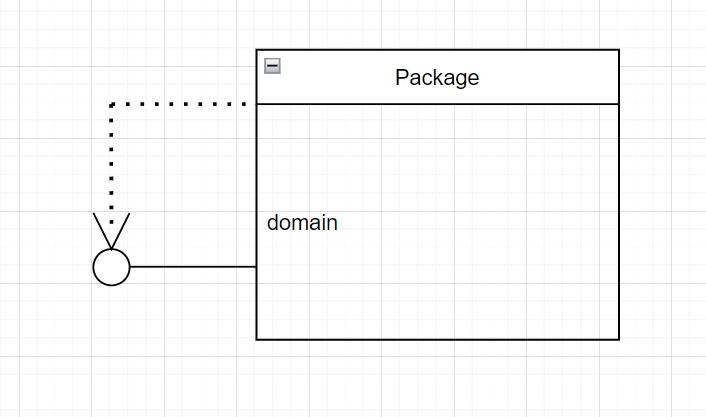
\includegraphics[scale=0.5]{images/first/layer.png}
\caption{ساختار الگوی \lr{Layered}}
\end{figure}
\subsubsection{الگوی \lr{Five Layer}}
\label{arch5LayerSec}
\begin{RTL}
الگوی معماری پنج‌لایه یک تطبیق خاص از \nameref{archLayerSec} است
که برای ساختاردهی بسیاری از سیستم‌های نهفته و بی‌درنگ
مفید است. این الگو معماری منطقی را به پنج لایه
تقسیم می‌کند که این امر به توسعه‌دهندگان کمک می‌کند
تا به راحتی ساختار سیستم‌های جدید را درک کنند.
این الگو از قابلیت انتقال بین پلتفرم‌های مختلف پشتیبانی
می‌کند و یک پلتفرم انتزاعی فراهم می‌کند که تطبیق برنامه‌ها
را آسان‌تر می‌سازد. در حالی که این الگو بسیاری از
مزایای \nameref{archLayerSec} را دارد، از جمله کارایی بالا به دلیل تعداد
کم لایه‌ها، ممکن است برای تجزیه کافی سیستم‌های پیچیده مناسب نباشد.
\end{RTL}
\subsubsection{الگوی \lr{Microkernel}}
\subsection{الگوی \lr{Channel}}
\subsubsection{الگوی \lr{Recursive Containment}}
\label{archRecContainSec}
\begin{RTL}
الگوی تجزیه و تحلیل بازگشتی برای مدیریت سیستم‌های بسیار پیچیده
با نیازمندی‌های فراوان مؤثر است. این الگو شامل شکستن سیستم به
اجزای مرتبط در سطوح مختلف جزئیات است، مانند استفاده از میکروسکوپ
با سطوح مختلف بزرگ‌نمایی. در هر سطح، اشیاء واسط‌هایی
برای همتایان خود فراهم می‌کنند و وظایف را به اجزای کوچک‌تر داخلی
تفویض می‌کنند، این تجزیه و تحلیل به صورت بازگشتی ادامه می‌یابد
تا هر بخش دارای مسئولیت ساده و متمرکز شود. این رویکرد امکان تجزیه
و تحلیل مقیاس‌پذیر را فراهم می‌کند و تأیید موارد استفاده بزرگ انتزاعی
را در هر مرحله ممکن می‌سازد و سطوح مختلفی از جزئیات رفتار سیستم را ارائه می‌دهد.
\end{RTL}
\subsubsection{الگوی \lr{Hierarchical Control}}
\label{archHierContSec}
\begin{RTL}
الگوی کنترل سلسله‌مراتبی \cite{ref4} یک
نسخه تخصصی از \nameref{archRecContainSec}
است که الگوریتم‌های پیچیده کنترلی را بین اجزای مختلف توزیع می‌کند.
این الگو از دو نوع واسط استفاده می‌کند:
واسط‌های کنترلی که نحوه دستیابی به رفتارها را نظارت و کنترل می‌کنند
و واسط‌های عملکردی که خدمات کنترل‌شده توسط واسط‌های دیگر را فراهم می‌کنند.
واسط‌های کنترلی کیفیت خدمات، مانند دقت و صحت، را تعیین می‌کنند
و سیاست‌های اجرایی را تنظیم می‌کنند. واسط‌های عملکردی رفتار مطلوب
را با استفاده از کیفیت خدمات و سیاست‌های تنظیم شده توسط واسط
کنترلی اجرا می‌کنند. این الگو با استفاده از نمودارهای حالت برای
هماهنگی اجزای زیرمجموعه و تجمیع اجزای جزء به کنترل‌کننده
از طریق ترکیب، ساختار سلسله‌مراتبی قابل تنظیم و مقیاس‌پذیری را
فراهم می‌کند. در این الگو، کنترل‌کننده وظیفه هماهنگی درخواست‌های
خدمات به عناصر جزء را دارد و اغلب از نمودارهای حالت برای نشان
دادن حالت‌های تنظیمات اجزای زیرمجموعه استفاده می‌کند. این روش
به ویژه زمانی مفید است که حالت‌های مختلف اجزای زیرمجموعه مستقل
نباشند و با استفاده از نمودارهای حالت و انطباق حالت‌ها، سازگاری میان اجزا حفظ شود.
\end{RTL}
\begin{figure}[h!]
\centering
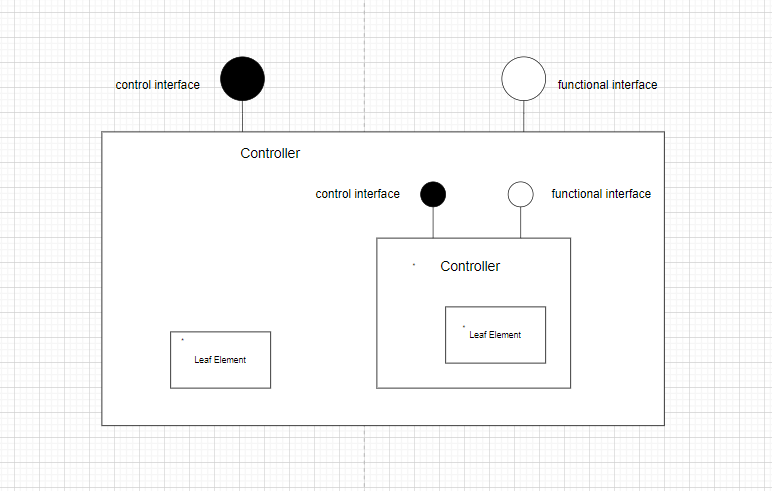
\includegraphics[scale=0.5]{images/first/hierarchical.png}
\caption{ساختار الگوی \lr{Hierarchical Control}}
\end{figure}
\subsubsection{الگوی \lr{Virtual Machine}}
\label{archVirtMachineSec}
\begin{RTL}
الگوی ماشین مجازی \cite{ref4} اولویت را
به قابلیت انتقال برنامه‌ها می‌دهد تا به کارایی
در زمان اجرا، و برای برنامه‌هایی که نیاز به اجرای روی پلتفرم‌های مختلف
دارند اما عملکرد حداکثری ضروری نیست، مناسب است.
برنامه‌ها برای یک ماشین انتزاعی نوشته می‌شوند و یک ماشین مجازی
نرم‌افزاری این دستورات را بر روی سخت‌افزار واقعی تفسیر می‌کند.
این الگو انتقال برنامه‌ها به محیط‌های جدید را ساده می‌کند،
زیرا فقط نیاز است ماشین مجازی برای پلتفرم هدف تطبیق داده شود.
اگرچه برنامه‌ها ممکن است کندتر از برنامه‌های کامپایل شده بومی اجرا
شوند، اما مزایای آن شامل ساده‌سازی انتقال و اندازه کوچکتر برنامه‌ها به
دلیل اشتراک کتابخانه‌ها در داخل ماشین مجازی است. با این حال، ماشین‌های
مجازی می‌توانند منابع زیادی مصرف کنند و ممکن است برای دستگاه‌های با
محدودیت حافظه مناسب نباشند. در چنین شرایطی ممکن است الگویی مانند
\nameref{archMicrokernelSec}
مناسب‌تر باشد.
\end{RTL}
\begin{figure}[h!]
\centering
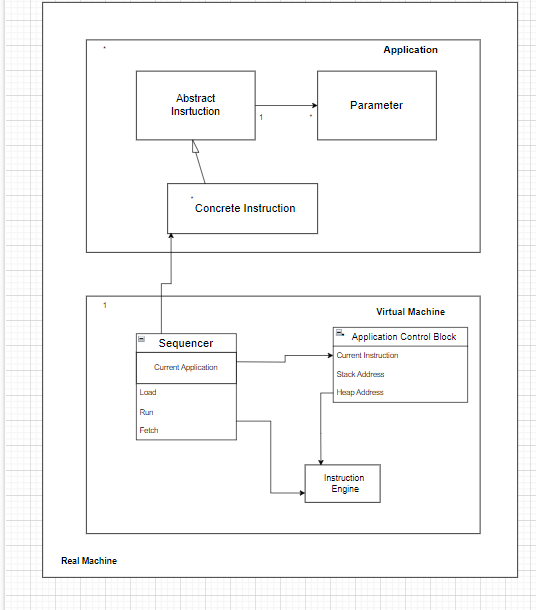
\includegraphics[scale=0.8]{images/first/virtual_machine.png}
\caption{ساختار الگوی \lr{Virtual Machine}}
\end{figure}
\subsubsection{معماری \lr{Component-Based}}
\label{archCompBasedSec}
\begin{RTL}
در \lr{UML}،
یک \lr{Component} یک اثر زمان اجرا و یک واحد قابل
جایگزینی اساسی در نرم‌افزار است
که مشابه یک شیء بزرگ‌مقیاس شامل اشیاء کوچکتری است که واسط آن را
پیاده‌سازی می‌کنند. \lr{Component}ها دارای کپسوله‌سازی قوی و
واسط‌های مستقل از زبان برنامه‌نویسی و کاملاً تعریف شده هستند.
سیستم‌های مبتنی بر \lr{Component}
که از این اشیاء بزرگ‌مقیاس به عنوان واحدهای معماری استفاده می‌کنند، از نگهداری
آسان، جداسازی عیوب، استقلال از زبان منبع، سادگی توسعه و قابلیت استفاده مجدد
بهره‌مند می‌شوند. \lr{Component}ها معمولاً اشیاء کوچکتری را
برای هدف رفتاری مشترک زمان اجرا جمع می‌کنند.
آنها دارای واسط‌های مبهم هستند، به این معنا که جزئیات
داخلی آنها از کلاینت مخفی است که این امر جایگزینی را تضمین می‌کند
اما ممکن است منجر به ناکارآمدی شود. الگوی معماری مبتنی بر مؤلفه معماری
سیستم را قوی و قابل استفاده مجدد فراهم می‌کند اما ممکن است به دلیل
استفاده از کل \lr{Component}ها حتی اگر فقط بخشی از عملکرد آنها
استفاده شود، منابع اضافی مصرف کند.
\end{RTL}
\subsubsection{الگوی \lr{ROOM}}
\subsection{الگوهای معماری هم‌زمانی}
\begin{RTL}

\end{RTL}
\subsubsection{الگوی \lr{Message Queuing}}
\subsubsection{الگوی \lr{Interrupt}}
\subsubsection{الگوی \lr{Guarded Call}}
\subsubsection{الگوی \lr{Rendezvous}}
\label{archConRendezSec}
\begin{RTL}
الگوی \lr{Rendezvous} \cite{ref4} نسخه
ساده‌تری از \nameref{archConGuardCallSec} است
که برای همگام‌سازی \lr{Thread}ها یا اجازه اشتراک‌گذاری داده‌ها بین آنها استفاده می‌شود.
این الگو از یک شیء \lr{Rendezvous} برای مدیریت همگام‌سازی استفاده می‌کند
که ممکن است شامل داده‌های اشتراکی یا فقط اعمال سیاست‌های همگام‌سازی باشد.
ساده‌ترین شکل آن، الگوی \lr{Thread Barrier} است که
\lr{Thread}ها را بر اساس تعداد مشخصی که در یک نقطه ثبت‌نام می‌کنند،
همگام می‌کند. پیش‌شرط‌ها برای همگام‌سازی باید برآورده شوند که
اغلب توسط ماشین‌های حالت در زبان‌های طراحی مانند \lr{UML} مدیریت می‌شوند.
این الگو تضمین می‌کند که \lr{Thread}ها منتظر می‌مانند
تا همه شرایط برآورده شود و سپس ادامه می‌دهند.
این الگو بسیار انعطاف‌پذیر است، برای نیازهای همگام‌سازی پیچیده کاربرد دارد
و به خوبی با تعداد زیادی از \lr{Thread}ها و شروط، مقیاس‌پذیر است.
(این الگو همان \nameref{scheduleRendezvousSec} است
که در \cite{ref1} گفته‌شده.)
\end{RTL}
\subsubsection{الگوی \lr{Cyclic Execution}}
\label{archConCyclicExecSec}
\begin{RTL}
الگوی \lr{Cyclic Execution} \cite{ref4} در سیستم‌های کوچک
یا سیستم‌هایی که نیاز به اجرای قابل پیش‌بینی دارند، به طور گسترده‌ای استفاده می‌شود.
این الگو با سادگی و پیش‌بینی‌پذیری خود، پیاده‌سازی آسانی دارد و برای محیط‌های محدود به
حافظه که استفاده از یک سیستم‌عامل بی‌درنگ به طور
کامل عملی نیست، مناسب است. این الگو وظایف
را در یک حلقه ثابت و تکراری اجرا می‌کند و اطمینان می‌دهد که هر
وظیفه به نوبت اجرا می‌شود. سادگی آن نقطه قوت اصلی آن
است، اما انعطاف‌پذیری ندارد و برای رسیدگی به رویدادهای با ضرب‌الاجل‌های
محدود بهینه نیست. وظایف نمی‌توانند در زمان اجرا اضافه یا
حذف شوند و سیستم به تنظیمات زمانی حساس است.
وظایف نادرست می‌توانند کل سیستم را مختل کنند و
الگو در شرایط بار زیاد ناپایدار است. با وجود محدودیت‌ها، برای
سیستم‌های کوچک و پایدار با دینامیک‌های قابل درک مناسب است.
(این الگو همان \nameref{scheduleCyclicExecSec} است که
در \cite{ref1} گفته‌شده.)
\end{RTL}
\subsubsection{الگوی \lr{Round Robin}}
\subsubsection{الگوی \lr{Static Priority}}
\subsubsection{الگوی \lr{Dynamic Priority}}
\label{archConDynPriorSec}
\begin{RTL}
الگوی \lr{Dynamic Priority}، اولویت وظایف را بر اساس فوریت
در زمان اجرا تنظیم می‌کند و معمولاً از استراتژی نزدیک‌ترین ضرب‌الاجل
استفاده می‌کند، جایی که وظیفه‌ای که نزدیک‌ترین ضرب‌الاجل را دارد
بالاترین اولویت را دریافت می‌کند. این روش بهینه است زیرا اگر
وظایف بتوانند توسط هر الگوریتمی زمان‌بندی شوند، می‌توانند توسط این
الگوریتم نیز زمان‌بندی شوند. با این حال، این الگو ناپایدار است،
به این معنی که پیش‌بینی اینکه کدام وظایف در شرایط بار زیاد شکست می‌خورند،
ممکن نیست. این الگو برای سیستم‌های پیچیده با وظایف تقریباً برابر از
نظر اهمیت و جایی که تحلیل استاتیک غیرممکن است، مناسب است.
در مقابل، \nameref{archConStaticPriorSec} برای سیستم‌های
ساده‌تر که وظایف و زمان‌بندی آن‌ها می‌تواند به دقت شناخته و برنامه‌ریزی شود،
بهتر است.
\end{RTL}
\section{الگوهای معماری هم‌زمانی}
\begin{RTL}

\end{RTL}
\subsection{الگوی \lr{Message Queuing}}
\subsection{الگوی \lr{Interrupt}}
\subsection{الگوی \lr{Guarded Call}}
\subsection{الگوی \lr{Rendezvous}}
\subsection{الگوی \lr{Cyclic Execution}}
\subsection{الگوی \lr{Round Robin}}
\subsection{الگوی \lr{Static Priority}}
\subsection{الگوی \lr{Dynamic Priority}}
\subsection{الگوهای معماری منابع}
\begin{RTL}
این دسته از الگوها که در \cite{ref4} نام برده شده‌اند،
به ما می‌گویند که چگونه می‌توان منابع را در یک سیستم بی‌درنگ نهفته
به اشتراک گذاشت و مدیریت کرد. در سیستم‌های نهفته، منابع بسیار محدود هستند
و این الگوها از این منظر بسیار حائز اهمیت هستند.
\end{RTL}
\subsubsection{الگوی \lr{Critical Section}}
\label{resourceCriticalSectionSec}
\begin{RTL}
(این الگو همان \nameref{scheduleCriticalRegSec} است
که در اینجا با نامی دیگر بیان شده‌است.)
\end{RTL}
\subsubsection{الگوی \lr{Priority Inheritance}}
\subsubsection{الگوی \lr{Highest Locker}}
\label{resourceHighestLockerSec}
\begin{RTL}
این الگو \cite{ref4}
به هدف کاهش وارونگی اولویت، سقف اولویتی برای هر منبع تعیین می‌کند.
وظیفه‌ای که مالک منبع است، در بالاترین سقف اولویت از بین همه
منابعی که در اختیار دارد اجرا می‌شود، به شرطی که وظایف
با اولویت بالاتر را مسدود کند. این الگو که نوعی تصحیح شده از
\nameref{resourcePriorInheritSec} است، وارونگی اولویت را به یک سطح
واحد محدود می‌کند، به شرطی که وظایف در حین داشتن منابع خود را معلق نکنند.
بر خلاف \nameref{resourcePriorInheritSec}، این الگو مانع از مسدودسازی
زنجیره‌ای در صورت پیش‌دستی وظیفه‌ای در حین مالکیت منبع می‌شود.
\end{RTL}
\begin{RTL}
این الگو سقف اولویت‌ها را در زمان طراحی با شناسایی بالاترین اولویت
بین کلاینت‌های هر منبع و افزودن یک واحد به آن تعریف می‌کند.
این الگو به طور موثری وارونگی اولویت را محدود می‌کند، اما می‌تواند منجر
به بلوکه شدن بیشتر در این سطح واحد نسبت به روش‌های دیگر شود.
به عنوان مثال، اگر یک وظیفه با اولویت پایین یک منبع با سقف اولویت بالا
را قفل کند، وظایف با اولویت متوسط ممکن است بیشتر مسدود شوند.
برای مدیریت این وضعیت، می‌توان افزایش اولویت را تا زمانی که
وظیفه دیگری تلاش برای قفل کردن منبع کند، به تعویق انداخت.
\end{RTL}
\begin{RTL}
این الگو از \lr{Deadlock} جلوگیری می‌کند،
به شرطی که تسک‌ها در حین داشتن منابع خود را معلق نکنند،
زیرا اولویت تسک قفل‌کننده بالاتر از دیگر کلاینت‌های منبع است.
با این حال، سربار محاسباتی در مدیریت سقف اولویت‌ها
و اطمینان از اجرای صحیح تسک‌ها بدون تعلیق وجود دارد.
\end{RTL}
\begin{figure}[h!]
\centering
\begin{tikzpicture}
    \lr{
    \umlclass[]{Scheluer}{
            \lr{}
        }{
            \lr{creatThread()}\\
            \lr{destroyThread()}\\
            \lr{blockThread()}\\
            \lr{unblockThread()}\\
            \lr{return()}
            }
            \umlclass[x=4.5, y=4]{TaskControlBlock}{
                \lr{NominalPriority}\\
                \lr{CurentPriority}\\
                \lr{StartAddr}\\
                \lr{EntryPoint}
            }{         
    }       
\umlclass[x=3.4, y=-2.5]{mutex}{}{  
}       
\umlclass[x=7.5, y=-2.5]{SharedResource}{
    \lr{proirityCelling}
}
{}       
    \umlclass[x=11, y=1]{AbstractThread}{ 
    }{  
        \lr{run()}      
}                  
\umlclass[x=11, y=-5]{ConcreteThread}{}{      
}       
    \umlunicompo[mult1=1, mult2=*, geometry=-|, anchor1=30, pos2=1.7]{Scheluer}{TaskControlBlock}
    \umlassoc[mult1=1, mult2=*]{Scheluer}{AbstractThread}
    \umlinherit[]{ConcreteThread}{AbstractThread}
    \umlassoc[mult1=1, mult2=1]{mutex}{SharedResource}
    \umluniassoc[mult1=*, mult2=1]{mutex}{Scheluer}
    \umluniassoc[mult1=1..*, mult2=*, pos1=0.33]{AbstractThread}{SharedResource}
    }  
\end{tikzpicture}
\caption{دیاگرام کلاس \lr{Highest Locker}}
\label{resourceHighestLockerClassDiag}
\end{figure}
\subsubsection{الگوی \lr{Priority Ceiling}}
\label{resourcePriorCeilSec}
\begin{RTL}
این الگو \cite{ref4}
یک روش پیچیده برای حل مشکلات وارونگی اولویت
و \lr{Deadlock} در سیستم‌های چندوظیفه‌ای بسیار قابل اعتماد است.
این الگو وارونگی اولویت و زمان‌های مسدود شدن وظایف را محدود می‌کند
و از وقوع \lr{Deadlock}های ناشی از رقابت بر سر منابع جلوگیری می‌کند.
اگرچه پیچیده‌تر و با سربار بیشتری نسبت به روش‌های دیگر مانند
\nameref{resourceHighestLockerSec} است، این الگو تضمین می‌کند
که یک وظیفه با اولویت بالا تنها می‌تواند توسط یک وظیفه با اولویت پایین‌تر
که مالک یک منبع مورد نیاز است مسدود شود.
\end{RTL}
\begin{RTL}
در این الگو، ممکن است یک وظیفه در حال اجرا نتواند
به یک منبع دسترسی پیدا کند حتی اگر آن منبع قفل نباشد،
اگر سقف اولویت آن منبع کمتر از سقف منابع سیستم فعلی باشد.
این امر با حذف احتمال وقوع شرایط انتظار حلقوی
به جلوگیری از \lr{Deadlock} کمک می‌کند.
با این حال، پیچیدگی و سربار محاسباتی افزوده باعث می‌شود این الگو کمتر توسط
سیستم‌عامل‌های بی‌درنگ تجاری پشتیبانی شود
و اغلب نیاز به افزونه‌های سفارشی برای پیاده‌سازی دارد.
\end{RTL}
\begin{figure}[h!]
\centering
\begin{tikzpicture}
    \lr{
    \umlclass[]{Scheluer}{
            \lr{systemPriorityCeiling}
        }{
            \lr{creatThread()}\\
            \lr{destroyThread()}\\
            \lr{blockThread()}\\
            \lr{unblockThread()}\\
            \lr{return()}
            }
            \umlclass[x=4.5, y=4]{TaskControlBlock}{
                \lr{NominalPriority}\\
                \lr{CurentPriority}\\
                \lr{StartAddr}\\
                \lr{EntryPoint}
            }{
    }       
\umlclass[x=3.4, y=-2.5]{mutex}{}{  
}       
\umlclass[x=7.5, y=-2.5]{SharedResource}{
\lr{proirityCelling} 
}
{}       
    \umlclass[x=11, y=1]{AbstractThread}{ 
    }{  
        \lr{run()}      
}                  
\umlclass[x=11, y=-5]{ConcreteThread}{}{      
}       
    \umlunicompo[mult1=1, mult2=*, geometry=-|, anchor1=30, pos2=1.7]{Scheluer}{TaskControlBlock}
    \umlassoc[mult1=1, mult2=*]{Scheluer}{AbstractThread}
    \umlinherit[]{ConcreteThread}{AbstractThread}
    \umlassoc[mult1=1, mult2=1]{mutex}{SharedResource}
    \umluniassoc[mult1=*, mult2=1]{mutex}{Scheluer}
    \umluniassoc[mult1=1..*, mult2=*, pos1=0.33]{AbstractThread}{SharedResource}
    }  
\end{tikzpicture}
\caption{دیاگرام کلاس \lr{Priority Ceiling}}
\label{resourcePriorCeilClassDiag}
\end{figure}
\subsubsection{الگوی \lr{Simultaneous Locking}}
\label{resourceSimLockingSec}
\begin{RTL}
(این الگو همان \nameref{scheduleSimLockingSec} است
که در \cite{ref1} بیان شده‌است.)
\end{RTL}
\subsubsection{الگوی \lr{Ordered Locking}}
\subsection{الگوهای معماری توزیع}
\begin{RTL}

\end{RTL}
\subsubsection{الگوی \lr{Shared Memory}}
\subsubsection{الگوی \lr{Remote Method Call}}
\subsubsection{الگوی \lr{Observer}}
\label{distrObserverSec}
\begin{RTL}
این الگو همان \nameref{HWObserverSec} است که در
\cite{ref1} گفته شده‌است؛ اما در این‌جا تعریف خود را به کاربردها
ارتباط با سنسور محدود نکرده‌است و در ساختار سیستم‌های توزیع‌شده معنا پیدا می‌کند.
در اینجا ساختار الگو کاملا مشابه \nameref{HWObserverSec} است؛
اما کلاس‌های کلاینت، هر کدام می‌توانند به صورت توزیع‌شده در آدرسی متفاوت
قرار داشته باشند.
\end{RTL}
\subsubsection{الگوی \lr{Data Bus}}
\label{distrDataBusSec}
\begin{RTL}
این الگو \cite{ref4}
\nameref{distrObserverSec} را با ارائه یک گذرگاه
مشترک گسترش می‌دهد که در آن چندین سرور اطلاعات خود را منتشر می‌کنند و چندین
کلاینت رویدادها و داده‌ها را دریافت می‌کنند.
این الگو برای سیستم‌هایی که سرورها و کاربران زیادی
باید داده‌ها را به اشتراک بگذارند مناسب است
و توسط گذرگاه‌های سخت‌افزاری مانند گذرگاه \lr{CAN} پشتیبانی می‌شود.
گذرگاه داده (\lr{Data Buss})
به عنوان یک مرکز مشترک برای به اشتراک‌گذاری داده‌ها در پردازنده‌ها
عمل می‌کند و به کلاینت‌ها اجازه می‌دهد که داده‌ها
را دریافت‌کنند یا برای دریافت آنها مشترک شوند.
این الگو به عنوان یک پروکسی با یک مخزن داده متمرکز عمل
می‌کند و می‌تواند اشیاء داده مختلف را مدیریت کند.
گذرگاه داده بسیار قابل گسترش است و انواع داده‌های جدید را
می‌توان بدون تغییر ساختار اصلی در زمان اجرا اضافه کرد.
با این حال، مکان گذرگاه داده باید از پیش تعیین شده باشد و مدیریت ترافیک
آن ممکن است ظرفیت گره را برای انجام کارهای دیگر محدود کند.
این الگو برای معماری‌های متقارن که سرورها در پردازنده‌های کمتر قابل
دسترس قرار دارند، مؤثر است.
\end{RTL}
\subsubsection{الگوی \lr{Proxy}}
\label{distrProxySec}
\begin{RTL}
الگوی پروکسی با استفاده از یک کلاس جایگزین، سرور واقعی را از کلاینت
انتزاع می‌کند و جداسازی و پنهان‌سازی ویژگی‌های خاص سرور
از کلاینت‌ها را امکان‌پذیر می‌سازد. این الگو در سیستم‌های نهفته که
سرورها ممکن است در فضای آدرس‌های مختلف باشند بسیار مفید است
و به کلاینت‌ها اجازه می‌دهد بدون اطلاع از مکان سرور با آن تعامل کنند.
این انتزاع طراحی مشتریان را ساده می‌کند و تغییرات سیستم را بدون تغییر
در تعاملات کلاینت-سرور تسهیل می‌کند. الگوی پروکسی به مدیریت شفافیت
ارتباطات کمک کرده و روش تماس با سرورهای راه دور را محصور می‌کند.
این الگو ترافیک ارتباطات را با کاهش تعداد پیام‌های ارسال شده
در شبکه و استفاده از سیاست اشتراک برای انتقال داده کاهش می‌دهد.
\end{RTL}
\subsubsection{الگوی \lr{Broker}}
\label{distrBrokerSec}
\begin{RTL}
الگوی بروکر یک نسخه متقارن از \nameref{distrProxySec} است که برای شرایطی
طراحی شده که مکان کلاینت و سرورها در زمان طراحی مشخص نیست. این الگو
یک بروکر را معرفی می‌کند، که یک مخزن ارجاع شیء است
و برای هر دو کلاینت و سرورها قابل مشاهده است و
به کلاینت‌ها در یافتن سرورها کمک می‌کند. این امکان استقرار
معماری‌های متقارن مانند تعادل بار پویا را فراهم می‌کند. الگوی بروکر
مسائل شفافیت ارتباطات را حل کرده و نیاز به دانش قبلی از مکان سرورها
را از بین می‌برد، که به افزایش مقیاس‌پذیری سیستم و پنهان‌سازی جزئیات زیرین
پردازنده‌ها و ارتباطات کمک می‌کند. اگرچه \lr{Object Request Broker}های
تجاری به خوبی از این الگو پشتیبانی می‌کنند، اما ممکن است منابع بیشتری
نسبت به سیستم‌های کوچکتر نیاز داشته باشند، که در این
موارد می‌توان از \lr{ORB}های کوچکتر یا پیاده‌سازی سفارشی استفاده کرد.
\end{RTL}
\subsection{الگوهای معماری امنیت و قابلیت اطمینان}
\begin{RTL}

\end{RTL}
\subsubsection{الگوی \lr{Protected Single Channel}}
\label{archSafeProtectSingleChSec}
\begin{RTL}
\lr{redundancy} کامل در سیستم‌هایی که امنیت در آن‌ها حیاتی است،
پرهزینه است، هم در تکرار سخت‌افزار و هم در توسعه آن.
این الگو یک جایگزین سبک برای افزایش ایمنی و قابلیت اطمینان است که با افزودن
چک‌های اضافی و مقداری سخت‌افزار اضافی این کار را انجام می‌دهد.
این الگو از یک کانال برای حسگر و تحریک استفاده می‌کند و خطاهای گذرا را
شناسایی و مدیریت می‌کند، اما خطاهای پایدار را نمی‌تواند مدیریت کند.
این رویکرد از نظر هزینه‌های تکراری و توسعه مقرون به صرفه است و برای سیستم‌هایی
که نیاز به عملکرد در حضور خطاهای پایدار ندارند یا حساس به هزینه هستند،
مناسب است. با این حال، به دلیل نقاطی که یک خطای منفرد می‌تواند باعث
از دست رفتن کل سیستم شود، برای همه سیستم‌های مرتبط با ایمنی مناسب نیست.
\end{RTL}
\subsubsection{الگوی \lr{Homogeneous Redundancy}}
\label{archSafeHomoRedundancySec}
\begin{RTL}
این الگو با استفاده از چندین کانال برای انجام وظایف، قابلیت اطمینان
سیستم را بهبود می‌بخشد. این کانال‌ها می‌توانند به صورت متوالی یا به صورت موازی
عمل کنند. این الگو از سیستم در برابر خطاهای تصادفی محافظت می‌کند و
در صورت خرابی به کانال پشتیبان سوئیچ می‌کند تا عملکرد مداوم را
تضمین کند. این الگو ساده طراحی می‌شود و برای خطاهای تصادفی مؤثر است
اما از خطاهای سیستماتیک محافظت نمی‌کند، زیرا هر خطای سیستماتیک در یک
کانال در کپی‌های آن نیز وجود خواهد داشت. در حالی که این الگو قابلیت
اطمینان بالایی در محیط‌های سخت ارائه می‌دهد، هزینه‌های بالاتری
به دلیل نیاز به سخت‌افزار تکراری دارد.
\end{RTL}
\subsubsection{الگوی \lr{Triple Modular Redundancy}}
\label{archSafeTripModRedunSec}
\begin{RTL}
الگوی تکرار سه‌گانه مدولار \lr{(TMR)} با استفاده از سه کانال
موازی برای پردازش تسک‌ها، مقایسه خروجی‌ها و اعمال قانون دو از سه
در صورت اختلاف، قابلیت اطمینان و ایمنی را افزایش می‌دهد. این الگو به
سیستم اجازه می‌دهد تا در حضور خطاهای تصادفی بدون از دست دادن داده‌های
ورودی یا نیاز به زمان اضافی برای تصحیح، به کار خود ادامه دهد.
در حالی که هدف آن محافظت در برابر خطاهای تصادفی مشابه
\nameref{archSafeHomoRedundancySec} است، عملیات موازی
\lr{TMR} آن را از نظر زمانی کارآمدتر می‌کند.
با این حال، بدون استفاده از کانال‌های ناهمگن، از خطاهای سیستماتیک
محافظت نمی‌کند. \lr{TMR} به دلیل تکرار سخت‌افزار هزینه بالایی دارد،
اما برای برنامه‌های بسیار حیاتی با نیاز به قابلیت اطمینان بالا
و بدون وضعیت ایمن ضروری است.
\end{RTL}
\subsubsection{الگوی \lr{Heterogeneous Redundancy}}
\subsubsection{الگوی \lr{Monitor-Actuator}}
\label{archSafeMonActSec}
\begin{RTL}
این الگو \cite{ref4} یک راهکار ایمنی مقرون‌به‌صرفه است که در سیستم‌هایی
با نیازمندی‌های دسترسی متوسط تا پایین و حالت ایمن تعریف‌شده استفاده می‌شود.
این الگو شامل یک حسگر مستقل است که کانال فعال‌سازی
را برای شناسایی خطاها نظارت می‌کند و اطمینان می‌دهد که
سیستم در صورت لزوم به حالت ایمن وارد می‌شود. این الگو شکل
خاصی از \nameref{archSafeHeteroRedundancySec} است که به جای تکرار
کامل کانال، نظارت را فراهم می‌کند. زمانی که سیستم می‌تواند با ورود
به حالت ایمن، خطاها را تحمل کند، مناسب است و
با کمترین تکرار اطمینان حاصل می‌شود که اگر یک کانال خراب شود،
کانال دیگر می‌تواند خطا را شناسایی کرده یا به کار خود ادامه دهد.
\end{RTL}
\subsubsection{الگوی \lr{Sanity Check}}
\label{archSafeSanityChkSec}
\begin{RTL}
این الگو در سیستم‌های نهفته بی‌درنگ یک روش سبک و کم‌هزینه
برای اطمینان از عملکرد معقول سیستم، حتی اگر کاملاً دقیق نباشد، است.
این الگو پوشش خطای حداقلی ارائه می‌دهد و برای شرایطی طراحی شده است که
کنترل دقیق برای ایمنی حیاتی نیست، اما اقدامات نادرست می‌توانند ضرر رسان باشند.
این الگو از حسگرهای ارزان‌قیمت و کم‌دقت برای شناسایی خطاهای قابل توجه
در عملکرد استفاده می‌کند و مطمئن می‌شود که سیستم در
صورت بروز انحرافات جزئی آسیب نمی‌بیند. این الگو یک نوع تغییر یافته از
\nameref{archSafeMonActSec} است که به یک حالت ایمن در صورت
بروز خطاهای بزرگ نیاز دارد و یک راه‌حل ساده و مقرون به صرفه
برای محافظت حداقلی فراهم می‌کند.
\end{RTL}
\subsubsection{الگوی \lr{Watchdog}}
\label{archSafeWatchDogSec}
\begin{RTL}
این الگو \cite{ref4}
یک روش سبک و کم‌هزینه برای اطمینان از عملکرد صحیح فرآیندهای
محاسبات داخلی است. برخلاف \nameref{archSafeSanityChkSec}
که خروجی سیستم را با استفاده از حسگرهای خارجی نظارت می‌کند،
الگوی \lr{Watchdog} بررسی می‌کند که محاسبات
به درستی و به موقع انجام شوند. این الگو پوشش خطای حداقلی ارائه می‌دهد
و عمدتاً خطاهای پایه زمانی و گیر افتادن احتمالی را شناسایی می‌کند.
این الگو اغلب با الگوهای ایمنی دیگر ترکیب می‌شود تا قابلیت اطمینان سیستم
را افزایش دهد، به‌ویژه در برنامه‌های حساس به زمان که محاسبات
باید ضرب‌الاجل‌های دقیقی را رعایت کنند.
\end{RTL}
\begin{figure}[h!]
\centering
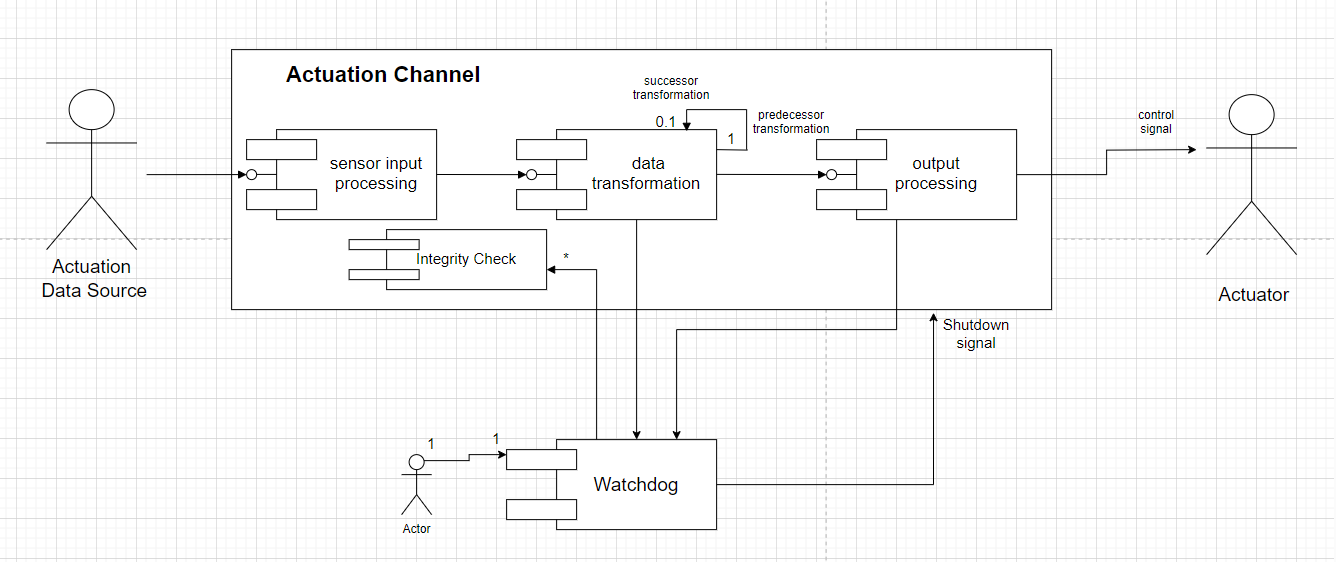
\includegraphics[scale=0.5]{images/third/watchdog.png}
\caption{ساختار الگوی \lr{Watchdog}}
\end{figure}
\subsubsection{الگوی \lr{Safety Executive}}
\label{archSafeSafetyExecSec}
\begin{RTL}
این الگو \cite{ref4}
برای سیستم‌هایی طراحی شده است که اقدامات ایمنی پیچیده‌ای دارند
و نمی‌توان آنها را به سادگی با خاموش کردن سیستم به دست آورد.
این الگو یک جزء مجری ایمنی معرفی می‌کند تا چندین کانال
و اقدامات ایمنی را مدیریت و هماهنگ کند و سیستم را از طریق
یک سری مراحل به وضعیت ایمن هدایت کند. این الگو به‌ویژه برای سیستم‌هایی
که با مواد خطرناک یا حالت‌های پرانرژی کار می‌کنند و خاموشی فوری می‌تواند
خطرناک باشد، مفید است. پیاده‌سازی این الگو پیچیده است و معمولاً
برای سیستم‌های بسیار حساس به ایمنی استفاده می‌شود و در
چنین محیط‌هایی حفاظت عالی در برابر خطا ارائه می‌دهد.
\end{RTL}
\begin{figure}[h!]
\centering
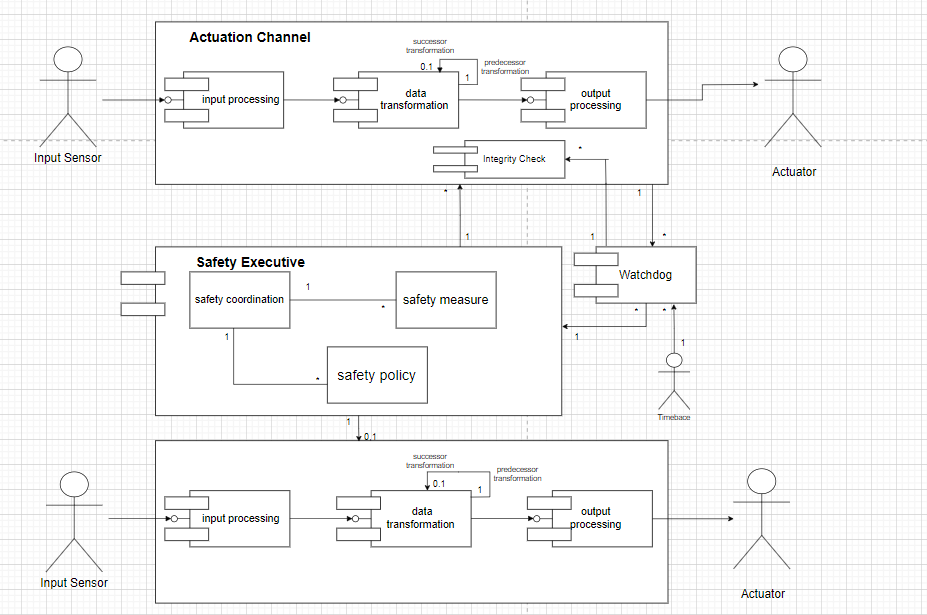
\includegraphics[scale=0.5]{images/third/safetyExec.png}
\caption{ساختار الگوی \lr{Safety Executive}}
\end{figure}
\section{الگوهای معماری امنیت و قابلیت اطمینان}
\begin{RTL}

\end{RTL}
\subsection{الگوی \lr{Protected Single Channel}}
\subsection{الگوی \lr{Homogeneous Redundancy}}
\subsubsection{الگوی \lr{Triple Modular Redundancy}}
\label{ArmoushHWTripModRedSec}
\begin{RTL}
(این الگو همان \nameref{archSafeTripModRedunSec} است
که در \cite{ref4} نوشته‌شده.)
\end{RTL}
\subsection{الگوی \lr{Heterogeneous Redundancy}}
\subsection{الگوی \lr{Monitor-Actuator}}
\subsection{الگوی \lr{Sanity Check}}
\subsubsection{الگوی \lr{Watchdog}}
\label{ArmoushHWWatchDogSec}
\begin{RTL}
(این الگو همان \nameref{archSafeWatchDogSec} است
که در \cite{ref4} نوشته‌شده.)
\end{RTL}
\subsubsection{الگوی \lr{Safety Executive}}
\label{ArmoushHWSafetyExecSec}
\begin{RTL}
(این الگو همان \nameref{archSafeSafetyExecSec} است
که در \cite{ref4} نوشته‌شده.)
\end{RTL}
\subsection{الگوهای نرم‌افزاری برای سیستم‌های \lr{Safety-Critical}}
\begin{RTL}

\end{RTL}
\subsubsection{الگوی \lr{N-Version Programming}}
\label{ArmoushSWNVerProgSec}
\begin{RTL}
الگوی \lr{N-Version Programming (NVP)} یک روش نرم‌افزاری تحمل خطا
است که بر تنوع نرم‌افزار و مخفی‌سازی خطاها متکی است.
این روش شامل ایجاد \lr{N} نسخه نرم‌افزاری معادل عملکردی
\lr{(N ≥ 2)} به‌صورت مستقل از مشخصات اولیه است.
این نسخه‌ها به‌طور موازی اجرا می‌شوند و وظیفه یکسانی را با
ورودی یکسان انجام می‌دهند تا \lr{N} خروجی تولید کنند.
در این الگو، یک رأی‌گیر برای تعیین خروجی صحیح با استفاده از نتایج
\lr{N} نسخه به کار می‌رود. \lr{NVP} برای سیستم‌های با ایمنی بسیار بالا مناسب است،
زمانی که نیاز به نرم‌افزار بسیار قابل اعتماد وجود دارد،
هزینه بالای توسعه نسخه‌های متعدد قابل تحمل است، تیم‌های مستقل برای توسعه نسخه‌های
مختلف موجود هستند و واحدهای سخت‌افزاری تکراری برای اجرای این
نسخه‌ها به‌صورت موازی قابل استفاده هستند. با این حال، \lr{NVP}
دارای معایبی مانند پیچیدگی و هزینه بالای توسعه نسخه‌های مستقل
و وابستگی به مشخصات اولیه است که می‌تواند خطاها را به تمامی نسخه‌ها
منتقل کند و ایمنی و قابلیت اطمینان سیستم را تحت تأثیر قرار دهد.
\end{RTL}
\subsubsection{الگوی \lr{Recovery Block}}
\subsubsection{الگوی \lr{Acceptance Voting}}
\subsubsection{الگوی \lr{N-Self Checking Programming}}
\label{ArmoushSWNSelfChkProgSec}
\begin{RTL}
این الگو \cite{ref5}
یک روش نرم‌افزاری تحمل خطای بسیار پرهزینه است
که بر تنوع طراحی نرم‌افزار و خود بررسی از طریق تکرار تأکید دارد.
این روش شامل تولید مستقل حداقل چهار ماژول نرم‌افزاری معادل
عملکردی از مشخصات اولیه است.
این نسخه‌ها به گروه‌هایی به نام اجزا مرتب می‌شوند،
که هر جزء شامل دو نسخه و یک الگوریتم مقایسه برای بررسی صحت نتایج است.
در طول اجرا، یک جزء به طور فعال خدمت مورد نیاز را ارائه
می‌دهد، در حالی که اجزای دیگر به عنوان یدک‌های آماده عمل می‌کنند.
برای اطمینان از تحمل خطا برای یک خطا، حداقل چهار
نسخه باید بر روی چهار واحد سخت‌افزاری اجرا شوند، که آن
را به پرهزینه‌ترین روش در مقایسه با سایر روش‌ها تبدیل
می‌کند. این الگو برای توسعه نرم‌افزار تحمل خطا برای
سیستم‌های بسیار بحرانی از نظر ایمنی مناسب است، جایی که نیاز
به نرم‌افزار بسیار قابل اعتماد است، هزینه بالای پیاده‌سازی‌های
متعدد قابل تحمل است، تیم‌های مستقل برای
توسعه نسخه‌های مختلف موجود هستند و امکان
استفاده از واحدهای سخت‌افزاری اضافی برای اجرای
این نسخه‌ها به صورت موازی وجود دارد. معایب اصلی این الگو
شامل وابستگی زیاد به مشخصات اولیه که ممکن است خطاها را به همه
نسخه‌ها منتقل کند، تعداد بالای نسخه‌های متنوع و
ماژول‌های سخت‌افزاری مورد استفاده در مقایسه با سایر
الگوها که همان تعداد خطا را تحمل می‌کنند،
و پیچیدگی توسعه \lr{N} نسخه‌ مستقل و معادل عملکردی است.
\end{RTL}
\subsubsection{الگوی \lr{Recovery Block with Backup Voting}}

\subsection{الگوهای ترکیبی سخت‌افزار و نرم‌افزار برای سیستم‌های \lr{Safety-Critical}}
\begin{RTL}
این دسته از الگوها که در \cite{ref5} آمده‌است، به صورت مشخص درباره
تکرار هیچ‌کدام از سخت‌افزار یا نرم‌افزار صحبت نمی‌کند.
\end{RTL}
\subsubsection{الگوی \lr{Protected Single Channel}}
\label{ArmoushMixProtSingleChSec}
\begin{RTL}
این الگو همان \nameref{archSafeProtectSingleChSec} است
که در \cite{ref4} آمده‌است.
\end{RTL}
\subsubsection{الگوی \lr{3-Level Safety Monitoring}}
\label{ArmoushMix3LvlSafeMonSec}
\begin{RTL}
این الگو \cite{ref5}
یک ترکیب از \nameref{ArmoushHWMonActSec}
و \nameref{ArmoushHWWatchDogSec} است که برای برنامه‌هایی
مناسب است که نیاز به مانیتورینگ ایمنی مداوم دارند و شامل یک حالت
ایمن در صورت خرابی هستند، بدون اینکه به سخت‌افزارهای تکراری
زیادی نیاز داشته باشند. این الگو شامل یک کانال سخت‌افزاری
واحد است که به سه سطح تقسیم می‌شود: سطح عملکرد،
مانیتورینگ و کنترل. سطح عملکرد زیربرنامه‌ای را برای
انجام عملکرد مورد نظر اجرا می‌کند، سطح مانیتورینگ سطح عملکرد
را نظارت می‌کند و سطح کنترل سطح مانیتورینگ و کل کانال
سخت‌افزاری را کنترل می‌کند. علاوه بر این، یک \lr{Watchdog} که
از طریق پیام‌های دوره‌ای با سطح کنترل ارتباط برقرار می‌کند،
برای بازنشانی سیستم به حالت ایمن در صورت خرابی استفاده می‌شود.
\end{RTL}
\begin{RTL}
این الگو برای توسعه سیستم‌های نهفته با یک حالت ایمن یا اقدام
اصلاحی مشخص و بدون تکرار سخت‌افزاری مناسب است.
هدف آن بهبود ایمنی سیستم تعبیه شده با هزینه معقول
در حضور خرابی در سیستمی با حالت ایمن است.
علاوه بر این، چگونه می‌توان سطح ایمنی مورد نیاز را حفظ کرد و
اطمینان حاصل کرد که سیستم آسیبی وارد نمی‌کند،
زمانی که انحرافی در خروجی \lr{Acutator}ها از نقطه تنظیم فرمان وجود دارد.
عیب اصلی این الگو این است که شامل یک کانال سخت‌افزاری واحد
است؛ بنابراین، نمی‌توان از آن برای تحمل خرابی‌های سخت‌افزاری
در برنامه‌هایی با نیازهای بالای قابلیت اطمینان و دسترسی استفاده کرد.
\end{RTL}
\section{مراجع}
\renewcommand{\section}[2]{}%
\begin{thebibliography}{1}
    
\bibitem{ref1}
\lr{Douglass, Bruce Powel. Design patterns for embedded systems in C: an embedded software engineering toolkit. Elsevier, 2010.}
\bibitem{ref2}
\lr{Zalewski, Janusz. "Real-time software architectures and design patterns: Fundamental concepts and their consequences." Annual Reviews in Control 25 (2001): 133-146.}
\bibitem{ref3}
\lr{Gamma, Erich, et al. "Design patterns: Abstraction and reuse of object-oriented design." ECOOP’93—Object-Oriented Programming: 7th European Conference Kaiserslautern, Germany, July 26–30, 1993 Proceedings 7. Springer Berlin Heidelberg, 1993.}
\bibitem{ref4}
\lr{Douglass, Bruce Powel. Real-time design patterns: robust scalable architecture for real-time systems. Addison-Wesley Professional, 2003.}
\end{thebibliography}
% \include{part2.tex}




\end{document}